\chapter{Results}
\label{results}
In this chapter we will present the results and offer a possible interpretation.

\section{Preface}
While the problem instance is too big to find an optimal solution, the models have been given ample time to compute feasible qualitative routes. Unexpectedly, the subtour elimination model is less efficient than the polynomial model, even in smaller instances. Even more unexpectedly, the polynomial formulation seems to be more efficient than the custom Column Generational approach, finding better solutions in orders of magnitude less time.

We have run the models on two datasets each: one using the forecasted data and the other using the real data.
The polynomial and subtour elimination models have been time-limited by the memory of the calculator, they seem to consume far more than what the running computer had to offer, thus their times are lower than those for column generation.


\section{Data}
The data collected by running each of the models can be summarized in the following table, we remind that the models were not run to conclusion but were limited by the capabilities of the available machine.

\begin{tabular}{ |p{2cm}||p{1.5cm}|p{1cm}|p{1.6cm}|p{1.4cm}|p{1,5cm}|p{1.5cm}|p{1.7cm}|  }
  \hline
  Model & Data & Time & Upper Bound & Lower Bound & Initial Lower Bound & Explored nodes & Generated Columns /Rows \\
  \hline
  Col. Gen. & Forecast & 11h & 12275.91 & 10653.04 & 10624.35 & 192295 & 302000 \\
  Col. Gen. & Real & 22h & 11456.74 & 10573.27 & 10549.30 & 363886 & 766420 \\
  Poly. & Forecast & 8h$^\dagger$ & 11223.83 & 4794.40 & 4034.81 & 4977643 & - \\
  Poly. & Real & 5h$^\dagger$ & 11354.86 & 4761.03 & 4033.18 & 4670016 & - \\
  Sub. Elim. & Forecast & 4h$^\dagger$ & 40474.66 & 4146.30 & 3931.12 & 141979 & 19452 \\
  Sub. Elim. & Real & 4h$^\dagger$ & 40474.66 & 4204.66 & 3931.12 & 138154 & 19473 \\
  \hline
\end{tabular}

We highlighted with $\dagger$ the models that had to be terminated for memory scarcity.

The best routes computed by the polynomial and column generation models at their time of termination are displayed in Figure~\ref{fig:res-colgen-avg}, Figure~\ref{fig:res-colgen-real}, Figure~\ref{fig:res-poly-avg} and Figure~\ref{fig:res-poly-real}. The subtour elimination approach did not generate intermediate results, as such it is impossible to find a comparable route.

The unprocessed information we used to compute summaries and visualizations can be found in the "logs" folder provided with the project.

\section{Discussion}
As can be observed, the polynomial model consistently yields superior results in significantly less time compared to our Branch and Price method. This observation is a testament to the impressive work done by the Gurobi team in developing Mixed Integer Programming (MIP) solving solutions that can efficiently handle even the most straightforward problem formulations.

It is worth noting, however, that we may have achieved even better results had we implemented more efficient subproblem formulations. With the benefit of hindsight, we recognize that given the number of clients required, a metaheuristic solution might have been a more appropriate approach. Nonetheless, the results obtained through our selected approach provide valuable insights into the problem and pave the way for further optimization efforts in the future.



\begin{figure}[tb]
    \centering
    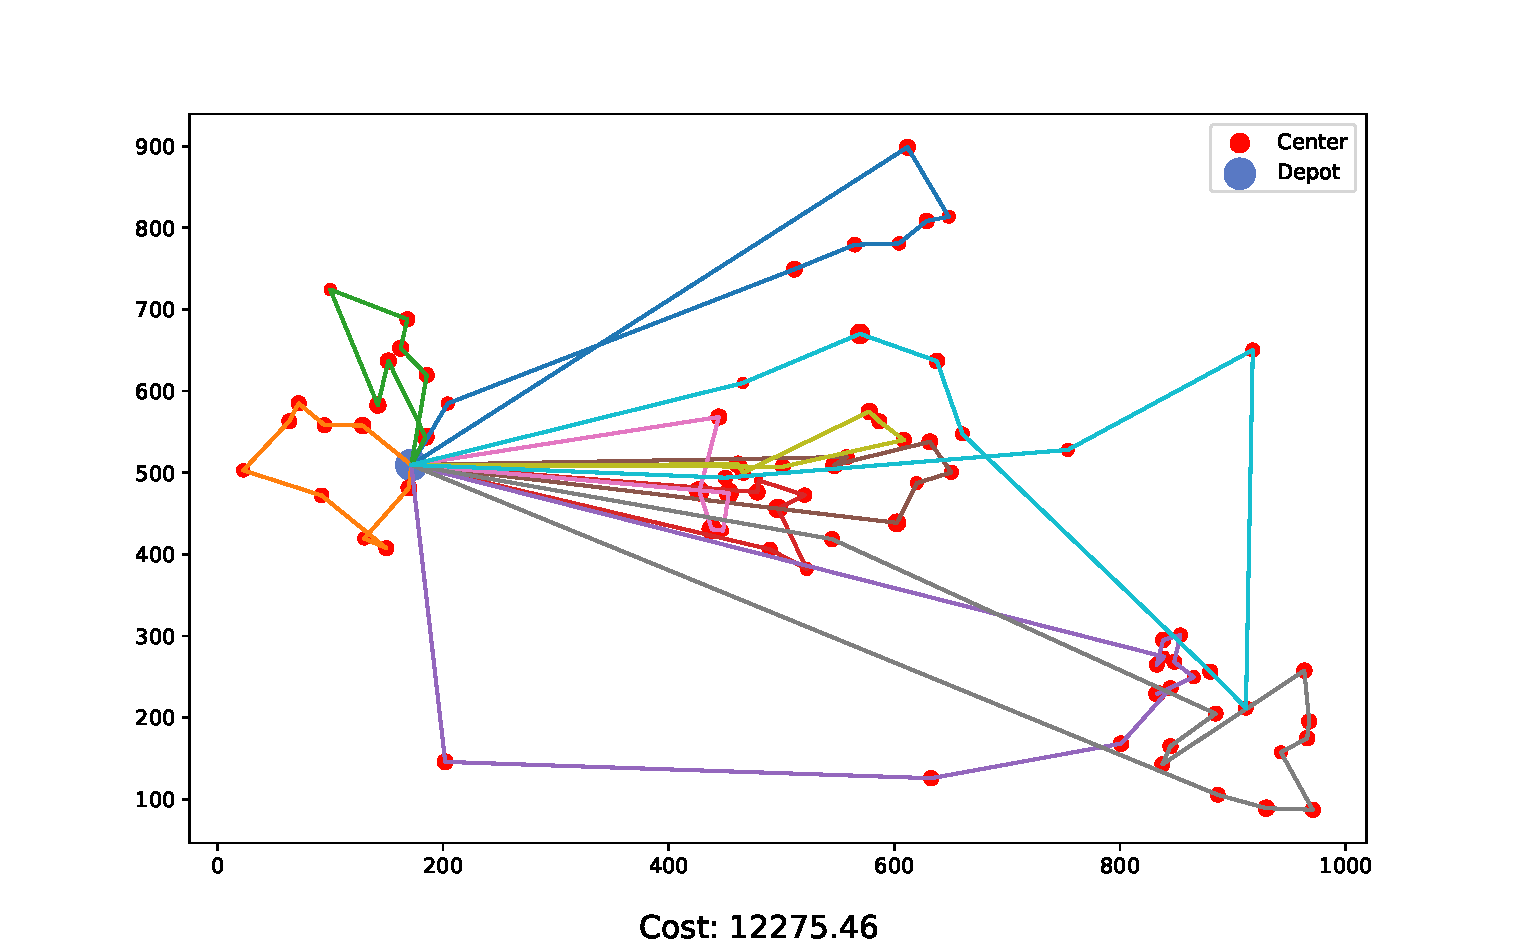
\includegraphics[width=1\columnwidth]{figures/results_colgen_avg.pdf}
    \caption{method: column generation, data: average, runtime: 11h}
  \label{fig:res-colgen-avg}
\end{figure}

\begin{figure}[tb]
    \centering
    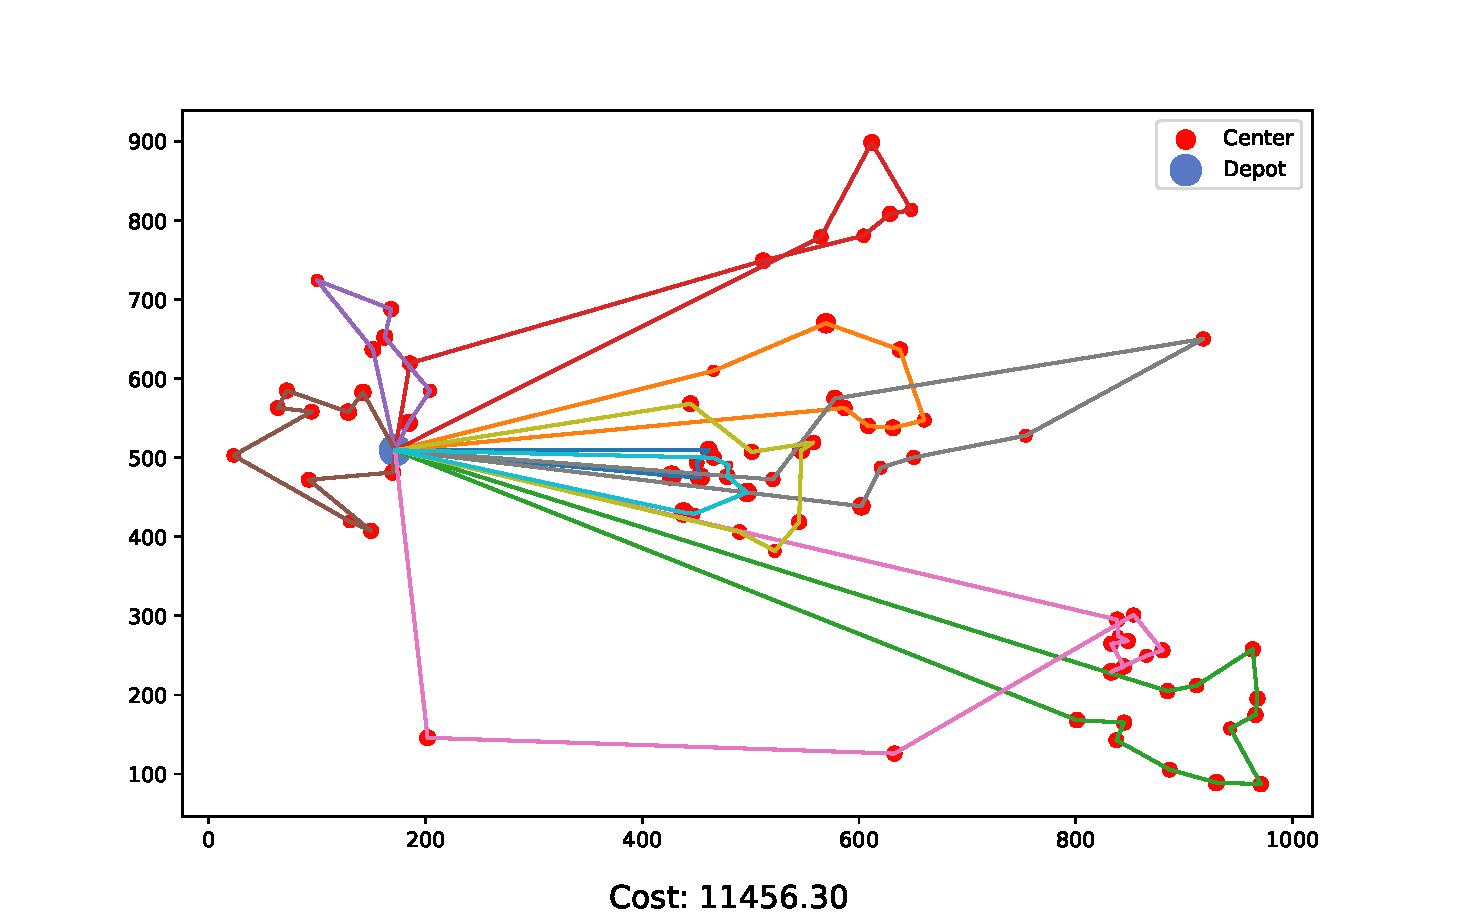
\includegraphics[width=1\columnwidth]{figures/results_colgen_real.pdf}
    \caption{method: column generation, data: real, runtime: 22h}
  \label{fig:res-colgen-real}
\end{figure}

\begin{figure}[tb]
    \centering
    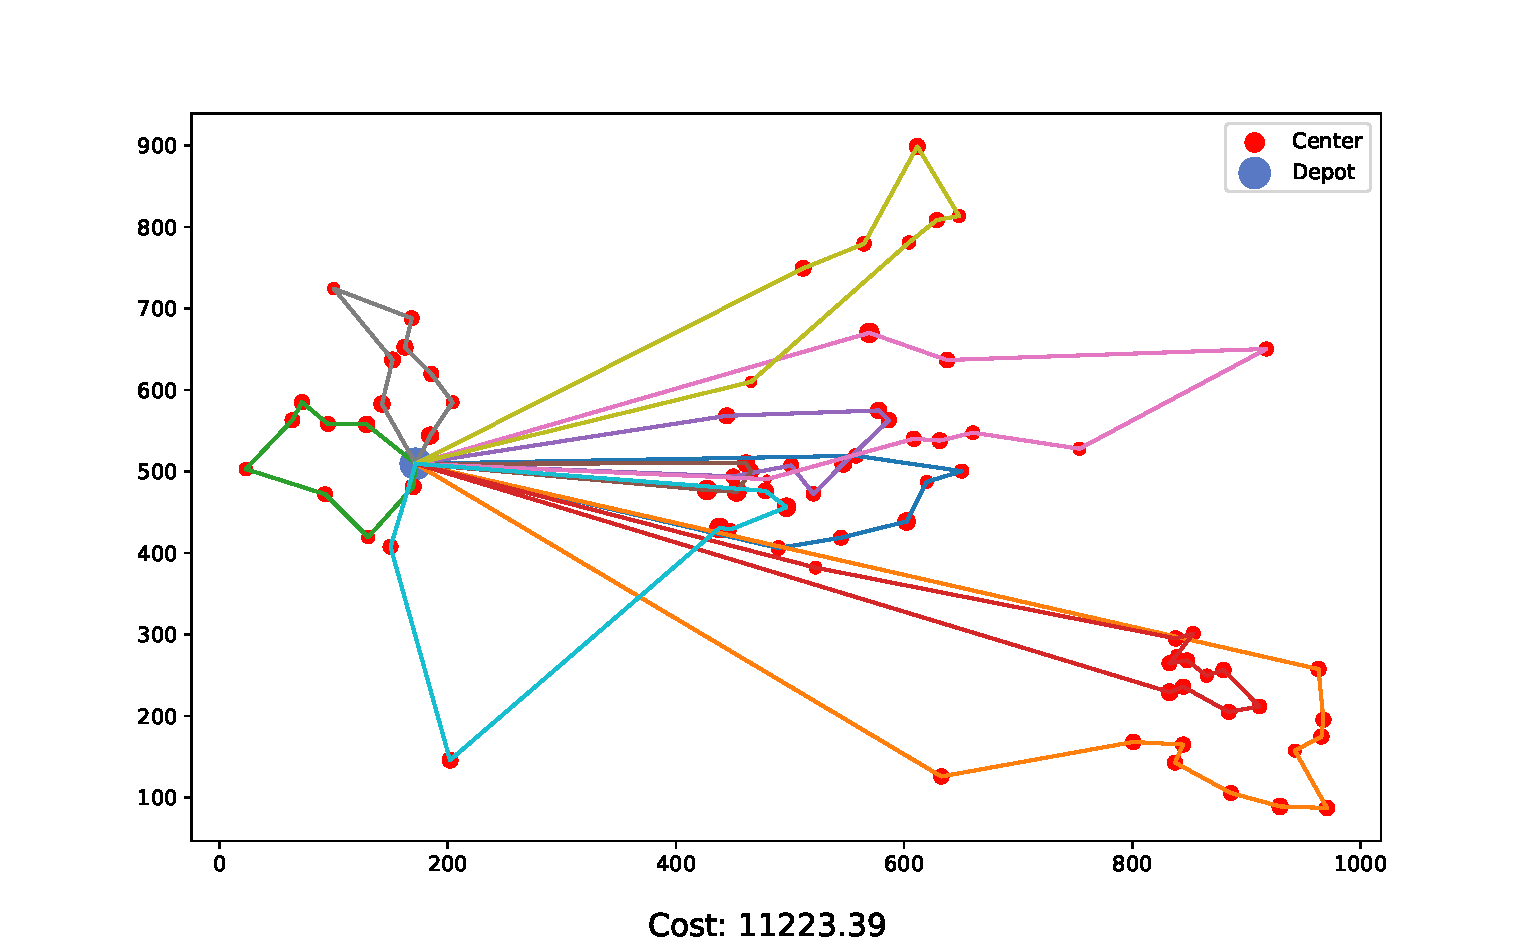
\includegraphics[width=1\columnwidth]{figures/results_poly_avg.pdf}
    \caption{method: polynomial, data: average, runtime: 7h}
  \label{fig:res-poly-avg}
\end{figure}

\begin{figure}[tb]
    \centering
    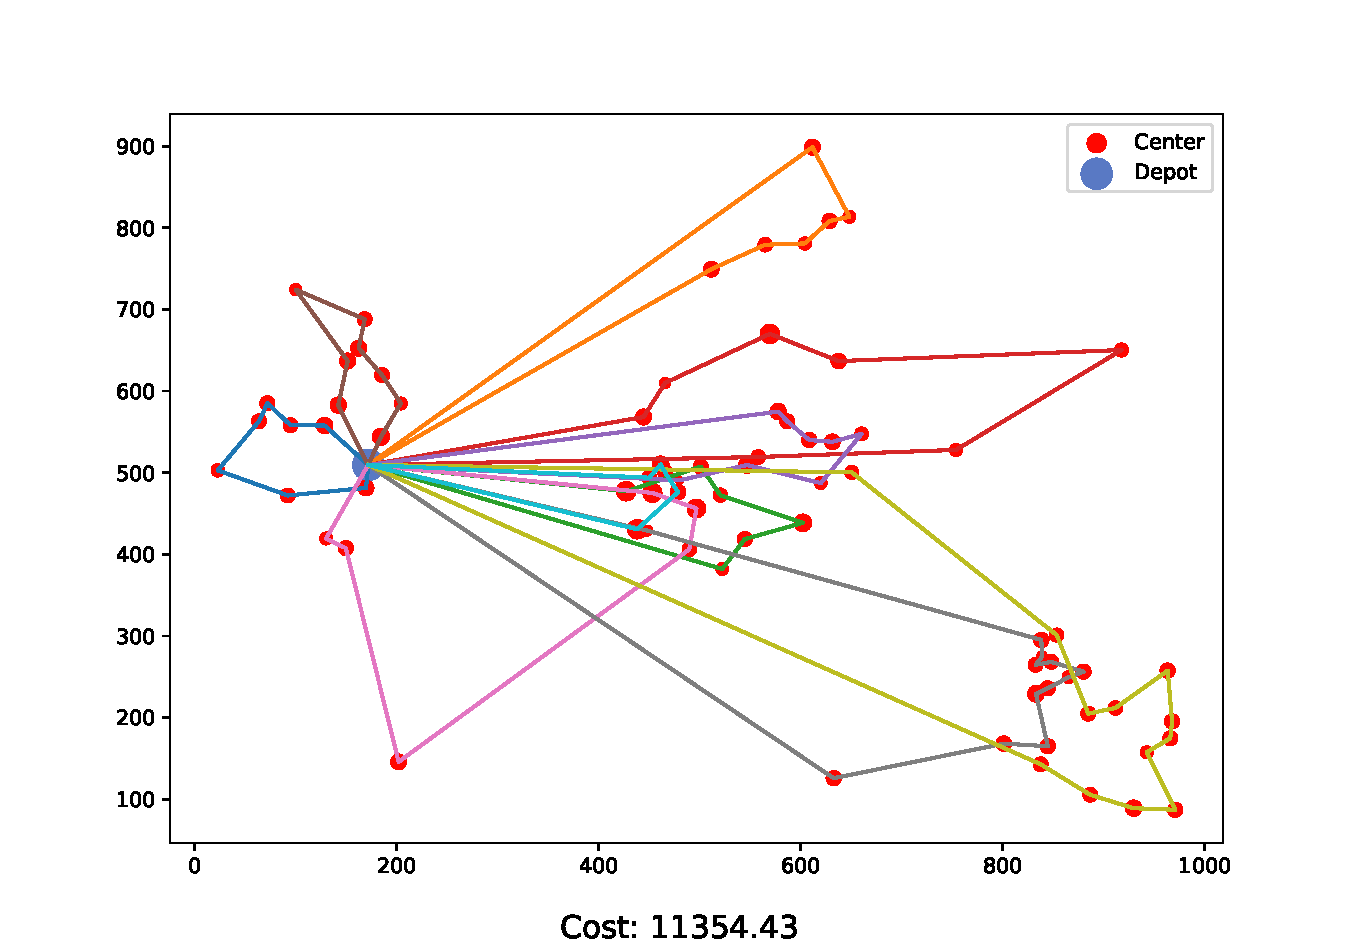
\includegraphics[width=1\columnwidth]{figures/results_poly_real.pdf}
    \caption{method: polynomial, data: real, runtime: 5h}
  \label{fig:res-poly-real}
\end{figure}
